\documentclass[a4paper,11pt]{article}
\usepackage{graphicx}
\usepackage{wrapfig}
\usepackage[a4paper, inner=3cm, outer=3cm, top=3cm, bottom=3cm, offset=0cm]{geometry}
\author{Kenneth Cross : 009200022
        \\Brendan Donahue : 007597252
        \\Mason Itkin : 007777029
        \\CMPE 130 : Tue - Thur : 1500
        \\San Jose State University}
\title{\textbf{Scheduling Algorithm}}
\date{\today}

\begin{document}
\pagenumbering{gobble}
\maketitle
\newpage
\tableofcontents
\newpage
\pagenumbering{arabic}
\setcounter{page}{1}

\newpage

\section{Methodology}

1) Staff Generation: Stored in a possibility matrix
2) Staff Optimization
3) Schedule Based on Staff Optimization Sum
4) Schedule Satisfaction Optimization

Maximization Factors
* Localization: establish potential rhythms and patterns for objects
* Position Preference: establish staff shift preferences
* Employee Preference: establish a hierarchy of skill based labor and give preference of desirable shifts to skilled employees. 

Multiple Shift Additions: Morning, Afternoon, Graveyard aka MAG

\begin{wrapfigure}{r}{4.5cm}
    \includegraphics[height=10cm]{graph.eps}
    \caption{\small Algorithm Digraph}
\end{wrapfigure}

\section{Data Representations}

Incoming input is currently contained in two separate CSV files. 
One file contains employee availability where the position section is a preference as to how many times per week someone would like to perform that position. The other file contains what types of positions are required and how many of each for every day of the week.


\end{document}
